\documentclass{report}

\usepackage{amssymb}
\usepackage{amsmath}
\usepackage{geometry}
\usepackage{textcomp}
\usepackage{booktabs}
\usepackage{enumitem}
\usepackage{amsfonts}
\usepackage{mathtools}
\usepackage{amsthm}
\usepackage{nicefrac, xfrac}
\usepackage{tikz}

\usetikzlibrary{positioning}



\mathcode`\*="8000{\catcode`\*\active\gdef*{\cdot}}
\DeclareMathOperator{\HO}{\mathcal{H}}
\DeclareMathOperator{\GO}{\mathcal{G}}

\theoremstyle{definition}
\newtheorem*{definition}{Definition}
\newtheorem*{theorem}{Theorem}
\newtheorem*{lemma}{Lemma}


\theoremstyle{remark}
\newtheorem*{remark}{Remark}
\newtheorem*{example}{Example}

\title{Numerical Methods - Lecture 1\\
{\Large University Leipzig}}
\date{April 2023}

\begin{document}

    \maketitle
    \tableofcontents


    \chapter{Number Systems}\label{ch:number-systems}
Standard decimal number:
\begin{align*}
    x = 1709.3_{10} = 1 * 10^{3} + 7 * 10^2 + 0*10^1+9*10^0+3*10^{-1}
\end{align*}
The $10$ indicates the base $b=10$.
Generally we can write a number as follows:
\begin{align*}
    x =\pm a_n*b^n+a_{n-1}*b^{n-1}+\ldots+a_0b^0+a_{-1}b^{-1}+\ldots
\end{align*}
Where $b \in \mathbb{N}$, $b>1$ and $a_i \in \{0,1, \dots, b-1\}$

If $b \leq 10$ the usually symbols can be used.
If $b>10$ new symbols are needed.
E.g.: hexadecimal ($b=16$):

\begin{center}
    \begin{tabular}{ c | c| c |c| c| c| c| c| c| c| c| c| c| c| c}
        1 & 2 & 3 & 4 & 5 & 6 & 7 & 8 & 9 & 10 & 11 & 12 & 13 & 14 & 15 \\
        \hline
        1 & 2 & 3 & 4 & 5 & 6 & 7 & 8 & 9 & A  & B  & C  & D  & E  & F  \\
    \end{tabular}
\end{center}


\section{Switching between different systems}\label{sec:switching-between-different-systems}
$1709_{10}$ in base $8$:
\begin{tabular}{ c c c c c }
    $8^0 = 1$ & $8^1 = 8$ & $8^2=64$ & $8^3=512$ & $8^4=4096$
\end{tabular}
\begin{align*}
    1709_{10} &= 3 * 512_{10} + 2 * 64_{10} + 5 * 8_{10} + 5_{10}\\
    &=3 * 8^3+2*8^2+5*8^1+5*8^0\\
    &=3255_8
\end{align*}
\emph{alternatively:} calculate in the new system:
\begin{flalign*}
    &10_{10} = 12_8\\
    &1709_{10} = 1 * {12_8}^3+7*{12_8}^2+0*{12_8}^1+9*{12_8}^0
\end{flalign*}
\emph{better alternative:} division with remainder:
\begin{align*}
    1709_{10}=3255_8=((3*8+2)*8+5)*8+5
\end{align*}
generally
\begin{align*}
    x = (\ldots (((a_nb+a_{n-1})b+a_{n-2})b+\ldots+a_1)b+a_0
\end{align*}
$a_0$ is remainder from division $x/b$
generally $a_i$ is the remainder from
\begin{align*}
    (\ldots((x-a_0)/b-a_1)/b\ldots-a_{i-1})/b
\end{align*}
\begin{alignat*}{2}
    1709:8 &= 213&|5\\
    213:8 &= 26     &|5\\
    26:8 &= 3       &|2\\
    3:8 &= 0       &|3\\
    1709_{10} &= 3255_8
\end{alignat*}


\section{Transformation of fractions}\label{sec:transformation-of-fractions}
Fraction $0.3_{10} = 3/10_{10}$
\begin{align*}
    3:12_8 = 0.2\overline{3146}_8\\
\end{align*}
\emph{better alternative:} repeated multiplication ($0 \leq x < 1$)
\begin{align*}
    x = (a_{-1}+(a_{-2}+(a_{-3}+\ldots)/b)/b)/b
\end{align*}
for example: $a_{-1}$ is position in front of the dot in $x*8$
\begin{flalign*}
    &0.3 * 8 = 2.4 \rightarrow 2\\
    &0.4 * 8 = 3.2 \rightarrow 3\\
    &0.2 * 8 = 1.6 \rightarrow 1\\
    &0.6 * 8 = 4.8 \rightarrow 4 \\
    &0.8 * 8 = 6.4 \rightarrow 6\\
    &0.4 * 8 = 3.2 \rightarrow 3 \\
    &\dots\\
    &0.3_{10}=0.2 \overline{3146}_8
\end{flalign*}


\section{Special Systems}\label{sec:special-systems}
The transformation becomes particularly simple if the base of one system is power or root of the other base. E.g.: $b = 2 = \sqrt[3]{8}$ from octal to binary
\begin{flalign*}
    1709_{10}   = &3*8^3+2*8^2+5*8^1+5\\
    = &3*2^9+2*2^6+5*2^3+5\\
    = &(0*2^2+1*2^1+^*2^0)*2^9+(0*2^2+1*2^1+0*2^0)*2^6\\
    &+(1*2^2+0*2^1+1*2^0)*2^3+(1*2^2+0*2^1+1*2^0)*2^0\\
    = &011010101101_2
\end{flalign*}

\begin{flalign*}
    &3_8 = 011_2\\
    &2_8 = 010_2\\
    &5_8 = 101_2
\end{flalign*}

From binary to hexadecimal:

\begin{flalign*}
    011010101101_2 &= 6AD_{16}\\
    0110_2 &= 6_{16}\\
    1010_2 = 10_{10} &= A_{16}\\
    1101_2 = 13_{10} &= D_{16}
\end{flalign*}






    \chapter{Number Systems}\label{ch:number-systems2}
In the computer, the smallest units of memory is the bit, which can assume
just 2 different states \\
\{0, 1\} \{on, off\}, \{true, false\} , not necessary numbers.
Larger units of memory are:
\begin{center}
    \begin{tabular}{ l l @{ }l}
        \toprule
        name & \multicolumn{2}{l}{value} \\
        \midrule
        Byte     & 8        & bits  \\
        Kibibyte & $2^{10}$ & bytes \\
        kilobyte & $10^3$   & bytes \\
        Mebibyte & $2^{20}$ & bytes \\
        Megabyte & $10^6$   & bytes \\
        \bottomrule
    \end{tabular}
\end{center}


\section{Integer numbers}\label{sec:integer-numbers}
Integer numbers can easily be represented.
The data ``standards`` are called ``data types`` and specify the size and value function.
E.g.: 1 byte unsigned integer;
\begin{center}
    \begin{tabular}{ l l }
        \toprule
        memory state & value  \\
        \midrule
        11111111     & 255    \\
        \ldots       & \ldots \\
        00000001     & 1      \\
        00000000     & 0      \\
        \bottomrule
    \end{tabular}
\end{center}

with negative numbers \textrightarrow{} 1 byte signed integer:
\begin{center}
    \begin{tabular}{ l l }
        \toprule
        memory state & value  \\
        \midrule
        01111111     & 127    \\
        \ldots       & \ldots \\
        00000001     & 1      \\
        00000000     & 0      \\
        11111111     & -1     \\
        11111110     & -2     \\
        11111101     & -3     \\
        \ldots       & \ldots \\
        10000000     & -128   \\
        \bottomrule
    \end{tabular}
\end{center}


\section{Floating point numbers (fractions)}\label{sec:floating-point-numbers-(fractions)}
Floating-point numbers are the product of number $m \in (0,1)$ called mantissa, an integer e power of
a base b (usually b = 2) and a sign s.
\begin{equation*}
    x = (-1)^s * m * b^e
\end{equation*}
{}
Datatype ``single precision`` / 32-bit float
\begin{center}
    \begin{tabular}{|l r| l @{\hspace{1cm}} r| l@{\hspace{2cm}} r|}
        \hline
        s & 1 bit & e & 8 bits & m & 23 bits\\
        \hline
    \end{tabular}
\end{center}
\begin{itemize}
    \item sign $(-1)^s$
    \item exponent e is an integer, but it is stored differently than ``normal`` integers - binary number is shifted by 127

    \begin{tabular}{l l l}
        \toprule
        memory state & binary number & value of e \\
        \midrule
        11111111     & 255           & 128        \\
        11111110     & 254           & 127        \\
        \ldots       & \ldots        & \ldots     \\
        100000000    & 128           & 1          \\
        01111111     & 127           & 0          \\
        \ldots       & \ldots        & \ldots     \\
        00000010     & 2             & -125       \\
        00000001     & 1             & -126       \\
        00000000     & 0             & -127       \\
        \bottomrule
    \end{tabular}

    The values $e = 127$ and $e = 128$ are not used in the usual way.
    Instead, they are reserved for special cases (e.g. $\pm 0$, $ \pm \infty$, signaling NaN)
    \item mantissa is a positive binary number.
    In order to achieve maximal precision e is chosen such that all positions of m are used (no leading zeros).
    The point is after the first digit.

    E.g.: 4-digit decimal mantissa:
    \begin{align*}
        310678 &\rightarrow 3.107 * 10^5 \\
        0.00043136 &\rightarrow 4.314 * 10^{-4}
    \end{align*}

    Hence, if $x \neq 0$ there is always a non-zero digit in front of the point.
    Since $b = 2$ this digit is a 1.
    It is therefore not stored, but set implicitly.
    (This is only not the case if $e=-127$)

    \begin{align*}
        m = 1 + \sum_{i = 1}^{23} m_i * 2^{-i}
    \end{align*}
\end{itemize}

The datatype double precision (float64, double)
\begin{center}
    \begin{tabular}{|l r| l @{\hspace{1cm}} r| l@{\hspace{2cm}} r|}
        \hline
        s & 1 bit & e & 11 bits & m & 52 bits\\
        \hline
    \end{tabular}
\end{center}
\begin{align*}
    e \in \{ -1023, \ldots, 1023 \} \\
    (-1022, 1024 \hbox{ reserved})
\end{align*}

\emph{Precision:} The relative precision with which a number
can be represented is determined by the number of bits of the mantissa $m \in [1, 2 )$.
23 bits \textrightarrow{} $2^{23} \approx 10^7$ different states of m \textrightarrow{} relative distance of a possible number x to its ``neighbor'' is $10^{-7}$.
double precision: 52 bits \textrightarrow $2^{-52} \approx 10^{-15}$

    \chapter{Stability and fixed-point theorem}\label{ch:stability-and-fixed-point-theorem}


\section{Stability}\label{sec:stability}
Consider
\begin{equation*}
    \int_0^1 \frac{x^{10} }{x+10} dx
\end{equation*}
This integral can be solved iteratively:
\begin{align*}
    y_n &= \int_0^1 \frac{x^n}{x+10} dx \\
    y_0 &= \int_0^1 \frac{1}{x+10} dx = \left[ \ln(x+10) \right]^1_0 = \ln\left( \frac{11}{10} \right) \approx 0.095310\\
    y_n + 10 * y_{n-1} &= \int_0^1 \frac{x^n+10*x^{n-1}}{x+10} dx = \int_0^1 x^{n-1} dx = \frac{1}{n}
\end{align*}
No we could use $y_n = \frac{1}{n}- 10 * y_{n-1}$ to obtain $y_1, \ldots{},  y_{10}$:
\begin{center}
    \begin{tabular}{r l}
        \toprule
        n  & $y_n$           \\
        \midrule
        0  & 0.0953102       \\
        1  & 0.0468982       \\
        2  & 0.0310181       \\
        3  & 0.0231520       \\
        4  & 0.0184804       \\
        5  & 0.0151955       \\
        6  & 0.0147117       \\
        7  & -0.00425944     \\
        8  & 0.167594        \\
        9  & -1.56483 \ldots \\
        10 & 15\ldots        \\
        11 & -157\ldots      \\
        \bottomrule
    \end{tabular}
\end{center}
If we use $y_n = \frac{1}{n}- 10 * y_{n-1}$, the initial error of $y_0$ grows like $10^n$ and since $y_n< y_{n+1}$, the error soon dominates.
This is unstable behaviour.

If we use
\begin{equation*}
    y_n = \frac{1}{10}*\left( \frac{1}{n+1}-y_{n+1} \right)
\end{equation*}
and start with the crude approximation $y_{30}=0$, the large error of $y_{30}$ is reduced by a factor of 10 with each iteration.
This is a stable algorithm.
\begin{center}
    \begin{tabular}{r l}
        \toprule
        n  & $y_n$      \\
        \midrule
        30 & 0          \\
        29 & 0.00333    \\
        28 & 0.00311    \\
        27 & 0.00324    \\
        \ldots \\
        20 & 0.00434704 \\
        \ldots \\
        0  & 0.0953102  \\
        \bottomrule
    \end{tabular}
\end{center}

A numerical algorithm is called stable, if the provided solution to a problem P is the exact solution to a Problem Q that can be derived from P by a slight variation of the input data.
Else it is called unstable.


\section{Fixed-point iteration and fixed-point theorem}\label{sec:fixed-point-iteration-and-fixed-point-theorem}
We search the root of $f(x) = 2x-\tan(x)$. $2x-\tan(x) = 0$ can be transformed into a fixpoint equation:
\begin{align*}
    &x = \Phi_1(x) = \frac{1}{2} \tan(x) \\
    &x = \Phi_2(x) = \arctan(2x)
\end{align*}
With $\hat{x} = \Phi(\hat{x})$
The idea of the fixed-point iteration is to create a sequence by repeated insertion in $\Phi$
\begin{equation*}
    x_{i+1} = \Phi(x_i)
\end{equation*}
which converges against $\hat{x}$

\begin{center}
    \begin{tabular}{r l l }
        \toprule
        $i$ & $x_{i+1}=\frac{1}{2}\tan(x)$ & $x_{i+1}=\arctan(2x_i)$ \\
        \midrule
        0   & 1.2                          & 1.2                     \\
        1   & 1.2861                       & 1.1760                  \\
        2   & 1.7084                       & 1.1688                  \\
        3   & -3.6108                      & 1.1666                  \\
        4   & {}!                          & 1.1659                  \\
        5   &                              & 1.1657                  \\
        6   &                              & 1.1656                  \\
        \bottomrule
    \end{tabular}
\end{center}
Consider the difference
\begin{equation*}
    |x_{i+1}-x_i| = |\Phi(x_i)-\Phi(x_{i-1})|
\end{equation*}

\emph{Definition:} Let $I=[a,b] \subset \mathbb{R}$ be an interval and $\Phi: I \to \mathbb{R}$ is a contraction on I if there is a $0 \leq \theta < 1$
such that $|\Phi(x)-\Phi(y)| \leq \theta |x-y|$.

Remark: $\theta$ is called Lipschitz constant $\to$ Lipschitz continuity if $0 \leq \theta < \infty$

\vspace{10mm}

\emph{Lemma:} If $\Phi: I \to  \mathbb{R}$ is continuously differentiable on I ($\theta \in C^1(I)$) then
\begin{equation*}
    \sup_{\substack{x,y \in I}} \frac{|\Phi(x)-\Phi(y)|}{|x-y|} = \sup_{\substack{z \in I}} \Phi'(x)
\end{equation*}
Proof: mean value theorem: For all $x,y \in I$, $x<y$ there is a $\xi \in [a,b]$ such that\\
$\Phi(x)-\Phi(y) = \Phi'(\xi)(x-y)$

\vspace{10mm}

\emph{Fixed-point theorem:} Let $I=[a,b] \subset \mathbb{R}$ be an interval and $\Phi: I \to I$ a contraction with Lipschitz constant $0 < \theta < 1$
Then:
\begin{enumerate}[label=(\roman*)]
    \item there is exactly one fixed-point $\hat{x}$ of $\Phi$, such that $\Phi(\hat{x}) = \hat{x}$
    \item For any initial value $x_0 \in I$ the fixed-point iteration $x_{i+1} = \Phi(x_i)$ converges against $\hat{x}$ with
    \begin{align*}
        |x_{i+1}-x_i| &\leq \theta *|x_i-x_{i+1}|\hbox{ and}\\
        |\hat{x}-x_i| &\leq \frac{\theta^i}{1- \theta} * |x_1-x_0|
    \end{align*}
\end{enumerate}
Proof: For all $x_0 \in I$
\begin{align*}
    |x_{i+1}-x_i|=|\Phi(x_{i+1})-\Phi(x_i)| &\leq  \theta * |x_i-x_{i-1}| \mbox{ therefore}\\
    |x_{i+1}-x_i| &\leq \theta^i*|x_1-x_0|
\end{align*}
Now we show that $x_i$ is a Cauchy sequence:
\begin{align*}
    |x_{i+k}-x_i| &\leq |x_{i+k}-x_{i+k-1}|+|x_{i+k-1}-x_{i+k-2}|+\ldots + |x_{i+1}-x_i|\\
    &\leq (\theta^{i+k-1}+\theta^{i+k-2}+\ldots+\theta^i)* |x_1-x_0|\\
    &= \theta^i*(\theta^{k-1}+\theta^{k-2}+\ldots+\theta^{0})*|x_1-x_0| \\
    &\leq \frac{\theta^i}{1-\theta}* |x_1-x_0|
\end{align*}
Therefore, $x_i$ is a Cauchy sequence which implies convergence. $\hat{x} = \lim_{\substack{i \to \infty}}x_i$ is also a fixpoint of $\Phi$, since:
\begin{align*}
    |\hat{x} - \Phi(\hat{x})|&=|\hat{x}-x_{i+1}+x_{i+1}-\Phi(\hat{x})|\\
    & = |\hat{x}-x_{i+1}+\Phi(x_i)-\Phi(\hat{x})|\\
    & \leq |\hat{x}-x_{i+1}| + |\Phi(x_i)-\Phi(\hat{x})|\\
    &  \leq |\hat{x}-x_i|+ \theta * |\hat{x}-x_i|\\
    &\to 0  \hbox{ for } i \to \infty
\end{align*}
Show that there is only one fixed-point by assuming the opposite.
If $\hat{x}$ and $\hat{y}$ are distinct fixed-points, then
\begin{equation*}
    0 \leq |\hat{x}-\hat{y}| = |\Phi(\hat{x})-\Phi(\hat{y})| \leq \theta * |\hat{x}-\hat{y}|
\end{equation*}
but $\theta < 1$, therefore this is only possible if $|\hat{x}- \hat{y}| = 0 \implies \hat{x} = \hat{y}$


\section{Rate of convergence}\label{sec:rate-of-convergence}
A sequence $x_i \in \mathbb{R}$ converges with order (at least) $P \leq 1$ against $\hat{x}$ if there is a constant $C>0$ such that
\begin{equation*}
    |x_{i+1}-\hat{x}| \leq C * |x_i-\hat{x}|^P
\end{equation*}
where if $P=1$ it is additionally required that $C>1$.
If $P=1$ we speak of linear convergence, if $P=2$ of quadratic convergence.

Alternatively the rate of convergence can also be defined through the inequalities of differences of adjacent elements of the sequence.
\begin{equation*}
    |x_{i+1}-x_i| \leq C * |x_i-x_{i-1}|^P
\end{equation*}
In general, the fixed-point iteration converges only linearly due to
\begin{equation*}
    |x_{i+1}-\hat{x}| \leq \theta * |x_i-\hat{x}|
\end{equation*}


\section{Newtons method (for root finding)}\label{sec:newtons-method-(for-root-finding)}
We are searching the root $\hat{x}$ of f, but now we also have access to the first order derivative $f'(x)$.
First order taylor expansion at current position x:
\begin{align*}
    f(x) &\approx f(x_i)+ f'(x_i)(x-x_i)\\
    f(\hat{x}) &= 0\\
    x_{i+1} &= x_i - \frac{f(x_i)}{f'(x_i)}
\end{align*}
This is a fixed-point equation with the iteration function $\Phi(x)= x - \dfrac{f(x)}{f'(x)}$

\vspace{10mm}

\emph{Example:} Calculation of the squareroot of C\@.
\begin{equation*}
    f(x)=x^2-C
\end{equation*}
In floating point calculation the exponent of C should be treated separately:
\begin{equation*}
    \sqrt {C} = \sqrt {m * 2^e} = \sqrt {m} * 2^{\frac{e}{2}}
\end{equation*}
and $\sqrt{2}$ (for odd e) be calculated once and stored
\begin{align*}
    \sqrt {m} &= ? \\
    f(x) = x^2-m &= 0 \\
    f'(x) &= 2x \neq 0
\end{align*}
Where $m\in[1,2)$ and $x \in \left[1, \sqrt{2}\right]$

\begin{align*}
    \Phi(x)&=x- \frac{f(x)}{f'(x)}= x- \frac{x^2-m}{2x}= \frac{x}{2}+ \frac{m}{2x} = \frac{1}{2} \left( x+ \frac{m}{x} \right)\\
    x_{i+1} &= \frac{1}{2}*\left(x_i+\frac{m}{x_i} \right)
\end{align*}

E.g: $m=1.96$
\begin{center}
    \begin{tabular}{r l l}
        \toprule
        i & $x_i$              & \# correct digits \\
        \midrule
        0 & 1                & $\leq 1$          \\
        1 & 1.48             & $=1$              \\
        2 & 1.420216         & $=3$              \\
        3 & 1.40000167       & $=6$              \\
        4 & 1.40000000000099 & $=12$             \\
        5 & 1.4              & $=15$             \\
        \bottomrule
    \end{tabular}
\end{center}
(number of correct digits approximately doubles every iteration $\to$ quadratic convervenge)

    \section{Rate of convergence for Newton's method}\label{sec:rate-of-convergence-for-newton's-method}
\begin{align*}
    0=f(\hat{x}) &= f(x_i) + f'(x_i)(\hat{x}-x_i)+\frac{1}{2}f(x_i)''(\hat{x}-x_i)^2+\ldots\\
    &=f(x_i)+f'(x_i)(\hat{x}-x_i)+\frac{1}{2}f(\xi)''(\hat{x}-x_i)^2 \text{ for }\xi \in [\hat{x}, x_i]\\
    \hat{x}\underbrace{-x_i+\frac{f(x_i)}{f'(x_i)}}_{x_{i+1}=x_i-\frac{f(x_i)}{f'(x_i)}} &= \frac{1}{2} \frac{f''(\xi)}{f'(x_i)}(\hat{x}-x_i)^2\\
    \\
    \hat{x}-x_{i+1}&=\frac{f''(\xi)}{2f'(x)}(\hat{x}-x_i)^2
\end{align*}
Hence if $f'$ is limited and if $\lvert f'(x) \rvert>\epsilon >0$ on an interval that contains the root,
we can expect quadratic convergence:
\begin{equation*}
    \lvert \hat{x}-x_{i+1} \rvert \leq M * \lvert \hat{x}-x_i \rvert^2
\end{equation*}


\section{Halley's method}\label{sec:halleys-method}
If the second derivative $f''(x)$ can be evaluated easily, then Halley's method can be useful.
Consider:
\begin{align*}
    g(x)&= \frac{f(x)}{\sqrt {\lvert f'(x) \rvert}}\\
    \lvert f'(x) \rvert &= \text{sign}(f'(x))*f'(x)\\
\end{align*}
Roots of f are roots of g and vice versa if $\lvert f'(x) \rvert < \infty$.
Now calculate the derivative of $g(x)$
\begin{align*}
    g'(x) &= \frac{f'(x) \sqrt{\lvert f'(x) \rvert}-f(x)*\frac{f''(x)}{2*\sqrt{\lvert f'(x) \rvert}}*\text{sign}(f'(x))}
    {\lvert f'(x) \rvert}\\
    &=\frac{f'(x)* \lvert f'(x) \rvert - \frac{1}{2} f(x)f''(x)*\text{sign}(f'(x))}{\lvert f'(x) \rvert * \sqrt {\lvert f'(x) \rvert}}\\
    &=\frac{f'(x)^2- \frac{1}{2}f(x)f''(x)}{f'(x)*\sqrt{\lvert f'(x) \rvert}}
\end{align*}
Apply Newtons method to $g(x)$
\begin{align*}
    x_{i+1} &= x_{i}- \frac{g(x_i)}{g'(x_i)}\\
    &=x_i-\cfrac{f(x_i)}{f'(x_i)-\cfrac{f(x_i)*f''(x_i)}{2*f'(x_i)}}=\cfrac{f(x_i)}{f'(x_i)*\left(1-\cfrac{f(x_i)*f''(x_i)}{2*f'(x_i)^2}\right)}
\end{align*}
This term can be considered to be a correction to Newtons method.
(Without calculation) Halley's method has cubic convergence.


\chapter{(Compolex) Roots of polynomials}\label{ch:(compolex)-roots-of-polynomials}
A Polynomial $P_n = a_n x^n+a_{n-1}x^{n-1}+\ldots+a_1 x+a_0$
should be evaluated according to
\begin{equation*}
    P_n = ((\ldots((a_n x+a_{n-1})x+a_{n-2})x+\ldots)x+a_1)x+a_0
\end{equation*}
which has better stability and requires fewer operations.


\section{Fundamental theorem of algebra}\label{sec:fundamental-theorem-of-algebra}
Let $P(z)=\sum_{k=0}^n a_k*z^k$ be a non-constant polynomial of order $n \geq 1$
and complex coefficients $a_k \in \mathbb{C}$.
Then $P$ has at least one root $\hat{z}$ with $P(\hat{z})=0$
If roots are counted according to their multiplicity, $P$ has $n$ roots.
If the roots $\hat{z_i}$ are known the polynomial can be written as
\begin{equation*}
    P(z)=a_n(z-\hat{z_1})(z-\hat{z_2})\ldots(z-\hat{z_n})
\end{equation*}
$\hat{z_i} = \hat{z_j}$ for $i \neq j$ is possible \textrightarrow{} two fold root in the representation of $P$.
\begin{equation*}
    P(z) = a_n(z-\hat{z_1})^{m_1}(z-\hat{z_2})^{m_2}\ldots (z-\hat{z_n})^{m_n}
\end{equation*}
Where the roots $z_i$ are pairwise distinct.
$m_i \in \mathbb{N}$ is called the multiplicity of the root $z_i$.
\begin{equation*}
    \sum_{i=1}^{k}m_i = n
\end{equation*}


\section{Müllers method}\label{sec:mullers-method}
Approximates the function by a parabolic (also works for non-polynomial functions)
If 3 initial values $x_1, x_2, x_3$ are given.
Then:
\begin{equation*}
    P(x)=a(x-x_3)^2+b(x-x_3)+c
\end{equation*}
\begin{align*}
    y_i &= f(x_i)\\
    y_1 &= a(x_1-x_3)^2+b(x_1-x_3)+c\\
    y_2 &=a(x_2-x_3)^2+b(x_2-x_3)+c\\
    y_3 &=c
\end{align*}
Task: Get the $a,b,c$ find root of $\tilde{P}(\tilde{x})=a\tilde{x}^2+b\tilde{x}+c$ and iterate again with
$x_4 = \hat{\tilde{x}}+x_3$

First we eliminate the parameter b to calculate a:
\begin{align*}
    \frac{y_1-c}{x_1-x_3}&=a(x_1-x_3)+b\\
    \frac{y_2-c}{x_2-x_3}&=a(x_2-x_3)+b\\
    \\
    a(x_1-x_2)&=\frac{y_1-c}{x_1-x_3}-\frac{y_2-c}{x_2-x_3}\\
    a&=\frac{(y_1-y_3)(x_2-x_3)-(y_2-y_3)(x_1-x_3)}{(x_1-x_3)(x_2-x_3)(x_1-x_2)}
\end{align*}
Now we can calculate the parameter b:
\begin{align*}
    b &= \frac{y_1-y_3}{x_1-x_3}-\frac{(y_1-y_3)(x_2-x_3)-(y_2-y_3)(x_1-x_3)}
    {(x_1-x_3)(x_2-x_3)(x_1-x_2)}*(x_1-x_3)\\
    &=\frac{(x_1-x_3)^2(y_2-y_3)-(x_2-x_3)^2(y_1-y_3)}{(x_1-x_3)(x_2-x_3)(x_1-x_2)}
\end{align*}
Now we calculate the root of $\tilde{p}$
\begin{equation*}
    x_4-x_3=\frac{-b \pm \sqrt{b^2-4ac}}{2a}
\end{equation*}
We select the solution that leads to the smaller $\lvert x_4- x_3 \rvert$ (The next estimate should be close to the current one).
Hence, the difference in the numerator and potential rounding issues.
Solution:
\begin{align*}
    x_4-x_3 = \hat{\tilde{x}} &= \cfrac{(-b \pm \sqrt {b^2-4ac})*(-b \mp \sqrt{b^2-4ac})}{2a*(-b \mp \sqrt {b^2-4ac})}\\
    &=\frac{b^2-(b^2-4ac)}{2a*(-b \mp \sqrt{b^2-4ac})}\\
    &=\frac{-2c}{b \pm \sqrt {b^2-4ac}}\\
    \text{Remember, we want} &\text{ to make $\lvert x_4-x_3 \rvert$ small}\\
    x_4-x_3&= \frac{-2c}{b+\text{sign}(b)\sqrt {b^2-4ac}}
\end{align*}
\begin{equation*}
    \begin{bmatrix}
        x_1 &x_2 &x_3\\
    \end{bmatrix}
    \to
    \begin{bmatrix*}
        y_1=f(x_1)\\
        y_2=f(x_2)\\
        y_3=f(x_3)
    \end{bmatrix*}
    \to
    \begin{bmatrix*}
        a &b &c
    \end{bmatrix*}
    \to
    \begin{bmatrix*}
        x_4
    \end{bmatrix*}
    \to
    \begin{bmatrix*}
        x_2 &x_3 &x_4
    \end{bmatrix*}
\end{equation*}

\section{Laguerre's Method}\label{sec:laguerres-method}
\begin{align*}
    p_n(x) = a_n(x-\xi_1)(x-\xi_2)\ldots(x-\xi_n)
\end{align*}
with unknown roots $\xi_i$
\begin{align*}
    p_n(\xi_i) &= 0\\
    \ln | p_n(x) | &= \ln(a_n) + \ln \lvert x- \xi_1 \rvert + \ln \lvert x- \xi_2 \rvert
    +\ldots + \ln \lvert x- \xi_n \rvert\\
    \frac{d}{dx} \left( \ln \lvert p_n(x)\rvert \right) = \frac{P_n'(x)}{p_n(x)}
    &= \frac{1}{x-\xi_1}+\frac{1}{x-\xi_2}+ \ldots + \frac{1}{x-\xi_n} \coloneqq \mathcal{G}(x)\\
    -\frac{d^2}{dx^2}(\ln \lvert p_n(x) \rvert)= \left( \frac{p_n''(x)}{p_n(x)}\right)^2-\frac{p_n''(x)}{p_n(x)}
    &= \frac{1}{(x-\xi_1)^2}+\frac{1}{(x-\xi_2)^2}+\ldots+\frac{1}{(x-\xi_n)^2} \coloneqq \mathcal{H}(x)
\end{align*}
$\mathcal{G}(x)$ and $\mathcal{H}(x)$ can be calculated since $p_n, p_n', p_n''$ are available.
Assumptions:
\begin{itemize}
    \item root closest to current estimate $x_i$ is $\xi_1$.
    Define as a distance $a=x_i-\xi_k$
    \item all other roots $\xi_2, \ldots, \xi_n$ have the same distance to $x_i$. $b=x_i-\xi_k$ for $k>1$
\end{itemize}
Now we can find an approximation for $\mathcal{G}, \mathcal{H}$:
\begin{align*}
    \mathcal{G}&= \frac{1}{a}+ \frac{n-1}{b}\\
    \mathcal{H}&= \frac{1}{a^2}+\frac{n-1}{b^2}\\
    b &= \cfrac{n-1}{\mathcal{G}-\cfrac{1}{a}}= \sqrt{\cfrac{n-1}{\mathcal{H}-\cfrac{1}{a^2}}}\\
    \cfrac{\left(\mathcal{G}-\cfrac{1}{a} \right)^2}{(n-1)^2} &= \cfrac{\mathcal{H}- \cfrac{1}{a^2}}{n-1}\\
    \\
    \GO^2-\frac{2}{a}\GO + \frac{1}{a^2}&=\left(\HO-\frac{1}{a^2} \right)(n-1)\\
    \frac{n}{a^2}-2 \GO \frac{1}{a}+ \GO^2- \HO(n-1)&=0\\
    \frac{1}{a^2}- \frac{2 \GO}{n}*\frac{1}{a}+\frac{\GO^2}{n}-\frac{\HO (n-1)}{n} &= 0\\
    \frac{1}{a}= \frac{\GO}{n} \pm \sqrt {\left(\frac{\GO}{n} \right)^2-\frac{\GO^2}{n}+ \frac{\HO (n-1)}{n}}\\
    a=\frac{n}{\GO \pm \GO^2(1-n)+ \HO (n(n-1))}
\end{align*}
$x_{i+1}=x_i -a$ We want a to be small.
For real $\GO$:
\begin{equation*}
    a = \frac{n}{\GO + \text{sign}(\GO) \sqrt {\GO^2(1-n)+ \HO n(n-1)}}
\end{equation*}
for complex values we choose sign that maximize the absolute value of the denominator.
\textrightarrow{} Cubic convergence in the proximity of a single root, reliable convergence to some root.

\section{Deflation}\label{sec:deflation}
If one root $\hat{x}$ of the polynomial $p_n$ has been found and the simplified polynomial
$Q_{n-1}= \sfrac{p_n}{(x-\hat{x})}$ can be calculated,
$Q_{n-1}$ can be evaluated since it is of a lower order and the roots of $Q_{n-1}$ are the remaining unknown roots.
One avoids to find $\hat{x}$ a second time.
This process can be repeated for each new root.
If $p_n$ has only real coefficients and if the root $\hat{x}$ is complex, then the complex
conjugate  $\bar{\hat{x}}$ is also a root of $p_n$.
In that case, we can divide by the product $(x-\bar{\hat{x}})(x-\hat{x})$ which
reduces the order of $p_n$ by 2.

Deflation is stable if one goes from absolutely small to large roots and starts
the polynomial division with the coefficients of highest order or if one goes
from large to small roots and starts division of the scalar term.
In any case, at the end all roots should be optimized using the original polynomial.

\section{Eigenvalue methods}\label{sec:eigenvalue-methods}
It can be shown that the polynomial $p_n = \sum_{i=0}^{n}a_i*x^i$ has the same roots as the characteristic polynom of:
\begin{equation*}
    A=
    \begin{pmatrix}
        \dfrac{a_{n-1}}{a_n} & \dfrac{a_{n-2}}{a_n} &\dots & \dfrac{a_0}{a_n}\\[0.9em]
        1 & 0 & \dots & 0\\[0.5em]
        0 & 1 & \dots & 0\\[0.5em]
        \vdots & \vdots &\ddots &0 \\[0.5em]
        0 &  \dots & 1 & 0
    \end{pmatrix}
\end{equation*}
Therefore, roots of $p$ are Eigenvalues of A and can be found using Eigenvalue-methods.



    \section{Aithen's Methods}\label{sec:aithen's-methods}
If one already uses an algorithm that shows linear convergence, Aithen's method might be useful to
accelerate convergence.
Linear convergence:
\begin{equation*}
    \lvert x_{i+1} - \hat{x} \rvert \leq C * \lvert x_i - \hat{x} \rvert
\end{equation*}
Assuming:
\begin{align*}
    \frac{ x_{i+1}-\hat{x} }{x_i - \hat{x}} &\approx
    \frac{ x_{i+2}-\hat{x}}{x_{i+1}-\hat{x}}\\
    (x_{i+1}-\hat{x})^2 &\approx (x_{i+2}-\hat{x})(x_i-\hat{x})\\
    x_{i+1}^2-2x_{i+1}\hat{x} &\approx x_i x_{i+2}-(x_i+x_{i+2})\hat{x}\\
    \hat{x}(x_i-2x_{i+1}+x_{i+2}) &\approx x_i x_{i+2}- x_{i+1}^2\\
    \hat{x} &\approx \frac{x_i x_{i+2}-x_{i+1}^2}{x_i-2x_{i+1}+ x_{i+2}}\\
    \hat{x}\approx\frac{x_i x_{i+2}-2x_i x_{i+1}+x_i^2-x_{i+1}^2+2x_i x_{i+2}-x_i^2}{x_i-2x_{i+1}+x_{i+2}}&= x_i-\frac{(x_{i+1}-x_i)^2}{x_{i+2}-2x_{i+1}+x_i}\\
\end{align*}
This method is also called $\Delta^2$-method.
\begin{align*}
    \Delta y_n &= y_{n+1}-y_n\\
    \Delta^2 y_n &= \Delta(\Delta y_n) = \Delta y_{n+1}-\Delta y_n = (y_{n+2}-y_{n+1})-(y_{n+1}-y_n)\\
    &=y_{n+2} -2y_{n+1}+y_n
\end{align*}
\begin{align*}
    \to \hat{x}\approx x_i - \frac{(\Delta x_i)^2}{\Delta^2 x_i}
\end{align*}


\chapter{Interpolation}\label{ch:interpolation}
Often instead of a function f only individual values $f(x_i)$ and
perhaps values of the derivatives $f'(x_i), f''(x_i)$ are available.
This is for instance the case if differential equations are being solved
numerically or with experimental data.
However, for experimental data, one typically uses fitting and not interpolation)
If one wants to obtain function values at intermediate position, integrate or
simply get a smooth representation, one has to interpolate.
That means one searches for a function $\varphi$ that agrees with $f$, $f'(x), \ldots$
at the nodes $x_i$:
\begin{align*}
    f(x_i)=\varphi(x_i)\\
    f'(x_i)=\varphi'(x_i)
\end{align*}


\section{Polynomial interpolation}\label{sec:polynomial-interpolation}
Simple problem (no derivatives): $y_i = f(x_i)$ with $i = 0, \ldots, n$ given,
looking for polynomial $P \in \mathbb{P}_n$ of degree $\leq n$ such that
$P(x_i) = y_i$

$P$ is unambiguous.
To show this, we assume the negation:
\begin{equation*}
    P, Q \in \mathbb{P}_n \text{ such that } P(x_i)=Q(x_i)=y_i\text{, for all } i = 0, \ldots, n
\end{equation*}
Then $P-Q$ is a polynomial of degree $\leq n$ with roots at
$x_0, x_1, \ldots x_n$.
But non-zero polynomials of degree $n$ have at most
exactly $n$ roots.
Hence, $P(x)-Q(x) = 0$
There are different methods for finding $P$, which can be associated with different
bases of the space of polynomials.

\subsection{Vandermonde-Matrix}\label{subsec:vandermond-matrix}
Using the monomial basis $\{ 1, x, x^2, x^3, \ldots, x^n\}$ $P(x_i) = y_i$ forms a
linear system of equations:
\begin{equation*}
    \begin{pmatrix*}
        1 &x_0 &x_0^2 &\ldots & x_0^n\\
        1 &x_1 &x_1^2 &\ldots & x_1^n\\
        \vdots \\
        1 & x_n & x_n^2&\ldots  &x_n^2
    \end{pmatrix*}
    *
    \begin{pmatrix*}
        a_0 \\
        \vdots\\
        a_n
    \end{pmatrix*}
    =
    \begin{pmatrix*}
        y_0\\
        \vdots\\
        y_n
    \end{pmatrix*}
\end{equation*}
The solution (inversion of $U$) is computationally expensive ($\propto n^3$) operations).

\subsection{Lagrange polynomials}\label{subsec:lagrange-polynomials}
An alternative basis is given by the Lagrange-polynomials $L_0, L_1, \ldots, L_n$ which implicitly are defined through $L_i(x_j) = \delta_{ij}$.\\
The explicit form is:
\begin{equation*}
    \prod_{j=0, j\neq i}^n \frac{x-x_j}{x_i-x_j}
\end{equation*}
The interpolating polynomial $P$ is obtained by superposition
\begin{align*}
    P(x) &= \sum_{i=0}^{n}y_i*L_i(x)\\
    \to P(x_j)&=\sum_{i=0}^{n} y_i L_i(x_j)= \sum_{i=0}^{n} y_i * \delta_{ij} = y_j\\
    \\
    P(x) &= y_0 L_0 (x) + y_1 L_1 (x) + y_2 L_2 (x) + \ldots\\
    P(x_2) &= y_0 \underbrace{L_0
        (x_2)}_0 + y_1 \underbrace{L_1 (x_2)}_0 + y_2  \underbrace{L_2 (x_2)}_{1} + y_3  \underbrace{L_3 (x_2)}_0, \ldots\\
\end{align*}
\begin{remark}
    The Lagrange polynomials form an orthonormal basis with respect
    to the inner product $\langle P, Q \rangle =\sum_{i=0}^{n} P(x_i) * Q(x_i)$
    \begin{align*}
        \to{} \langle P, L_i \rangle &= P(x_i)\\
        P = \sum_{i=0}^n \langle P, L_{i} \rangle L_i &= \sum_{i=0}^{n} P(x_i) L_i
        = \sum_{i=0}^{n} y_i L_i(x)
    \end{align*}
\end{remark}

\begin{example}
    \begin{equation*}
        f(x)= \frac{1}{x}
    \end{equation*}
    \begin{center}
        \begin{tabular}{l l l}
            \toprule
            $i$ & $x_i$ & $y_i$          \\
            \midrule
            0   & 2     & $\sfrac{1}{2}$ \\
            1   & 2.5   & $\sfrac{2}{5}$ \\
            2   & 4     & $\sfrac{1}{4}$ \\
            \bottomrule
        \end{tabular}
    \end{center}

    \begin{align*}
        L_0(x) &= \frac{(x-2.5)(x-4)}{(2-2.5)(2-4)}=(x-6.5)*x+10\\
        L_1(x) &= \frac{(x-2)(x-4)}{(2.5-2)(2.5-4)}=\frac{(-4x+24)x-32}{3}\\
        L_2(x) &= \frac{(x-2)(x-2.5)}{(4-2)(4-2.5)}= \frac{(x-4.5)x+5}{3}\\
        P=\sum_{i=0}^{2}y_i*L_i(x) &= \frac{1}{2}((x-6.5)x+10)+ \frac{2}{5}
        \left( \frac{(-4x+24)x-32}{3} \right)+\frac{1}{4}\left( \frac{(x-4.5)x+5}{3} \right)\\
        &=(0.05x-0.425)x+1.15
    \end{align*}
\end{example}

\subsection{Recursive determination of the interpolating polynomial / Neville's method}\label{subsec:recursive-determination-of-the-interpolating-polynomial-/-neville's-method}
Let $P_{m_0, m_1, \dots, m_k} (x)$ be the polynomial of degree $k$ that interpolates $f(x)$\\
at the nodes $x_{m_0}, x_{m_1},\ldots,x_{m_k}$
\begin{equation*}
    P(x)= \frac{(x_j-x)P_{0,1,\ldots, j-1, j+1, \ldots, n}(x)-(x_i-x)P_{0,1,\ldots, i-1, i+1, \ldots, n}(x)}{(x_j-x_i)}
\end{equation*}
is the polynomial of degree n that interpolates f at the nodes $x_0, \ldots, x_n$ (proof by plugging in).

Involves a lot of operations but is efficient if one is only interested in the value of the interpolating polynomial at one specific position $\hat{x}$.
Then $P_{1,2}(\hat{x})$, $P_{0,1,\ldots, n-1}(\hat{x})$, \ldots are just numbers.

\subsection{Newton's method}\label{subsec:newton's-method}
Newton basis: $N_0 (x) = 1$, $N_1(x) =(x-x_0)$, $N_2(x)=(x-x_0)(x-x_1)$, \ldots
\begin{align*}
    N_i(x)=\prod_{k=0}^{i-1}(x-x_k)\\
    \to P_{0,1,\ldots, i-1}(x)+c_i * N_i(x) = P_{0,1,\ldots, i}(x)\\
    \text{since } N_i(x_0)=N_i(x_1)=\ldots=N_i(x_{i-1})=0
\end{align*}
The problem becomes what is $c_i$?
effective determination through divided differences($f[\ldots]$). Polynomial of degree 0:
\begin{align*}
    P_i(x) &= f[x_i] \coloneqq f_i = f(x_i)\\
    P_{i, i+1} &= \frac{(x_i - x) P_{i+1}-(x_{i+1} P_i(x))}{x_i-x_{i+1}} =f[x_i]+(x-x_i)\underbrace{f[x_i, x_i+1]}_{=c}\\
    &=\frac{(x_i-x)f[x_{i+1}]-(x_{i+1}-x) f[x_i]}{x_i-x_i+1}\\
    f[x_i, x_{i+1}] &= \frac{(x_i-x)f[x_{i+1}]-(x_{i+1}-x) f[x_i]-(x_i-x_{i+1}) f[x_i]}{(x_i-x_{i+1})(x-x_i)}\\
    &= \frac{(x_i-x)f[x_{i+1}]-(x_i-x)f[x_i]}{(x_i-x_{i+1})(x-x_i)}=\frac{f[x_i]-f[x_{i+1}]}{x_i-x_{i+1}}
\end{align*}
Let the ($n-1$)th divided difference $f[x_0, \ldots, x_{n-1}]$ and $f[x_i, \ldots, x_n]$ be known.
\begin{align*}
    P(x)=P_{0, \ldots, n}(x)&=P_{0,1,\ldots, n-1}(x)+f[x_0, \ldots, x_n](x-x_0)(x-x_1)\ldots(x-x_{n-1}) \text{(\textasteriskcentered{})}\\
    P_{0,\ldots, n-1}(x)&=f[x_0]+f[x_0, x_1](x-x_0)+f[x_0,x_1,x_2](x-x_0)(x-x_1)+
    \ldots\\
    &\phantom{=}+f[x_0,\ldots, ]x_{n-1}(x-x_0)(x-x_1)\ldots(x-x_{n-2})\\
    P_{1,\ldots, n} &= f[x_1] + f[x_1, x_2](x-x_1)+f[x_1, x_2, x_3](x-x_1)(x-x_2)+\ldots\\
    &\phantom{=}+f[x_1, x_2, \ldots, x_n] (x-x_1)(x-x_2)\ldots (x-x_{n-1})\\
    P_{0,1,\ldots, n}(x) &= \frac{(x_0-x)P_{1,\ldots, n}(x)-(x_n-x)P_{0,\ldots, n-1}}{x_0-x_n} \text{(\textasteriskcentered{}\textasteriskcentered{})}\\
    &\text{compare coefficients of $x^n$ in (\textasteriskcentered{}) and (\textasteriskcentered{}\textasteriskcentered{})}\\
    f[x_0,\ldots, x_n]&=\frac{f[x_0, \ldots, x_n-1]-f[x_1, \ldots, x_n]}{x_0-x_1}
\end{align*}

    For $n+1$ data points $(x_i, f(x_i))$, $i = 0,1,\ldots, n$ with pairwise distinct $x_i$ there is exactly one interpolating polynomial $P(x)$
of degree $\leq n$ which is given by
\begin{align*}
    P(x) &= f[x_0]+f[x_0, x_1] (x-x_0) + f[x_0, x_1, x_2] (x-x_0)(x-x_1)+\\
    &\phantom{=}\ldots + f[x_0, x_1, \ldots, x_n] (x-x_0)(x-x_1)\ldots (x-x_{n-1})\\
\end{align*}
where the divided differences are given by
\begin{align*}
    f[x_i] = f(x_i)\\
    f[x_i, \ldots, x_{i+k}] = \frac{f[x_i, \ldots, x_{i+k-1}]-f[x_{i+1}, \ldots, x_{i+k}]}{x_i - x_{i+k}}
\end{align*}
Now we calculate the interpolating polynomials in the newton base, for previous example


\begin{center}
    \begin{tabular}{ccc}
        \toprule
        i & $x_i$ & $y_i$ \\
        \midrule
        1 & 2     & 1/2   \\
        2 & 2.5   & 2/5   \\
        3 & 4     & 1/4   \\
        \bottomrule
    \end{tabular}
\end{center}


\begin{center}
    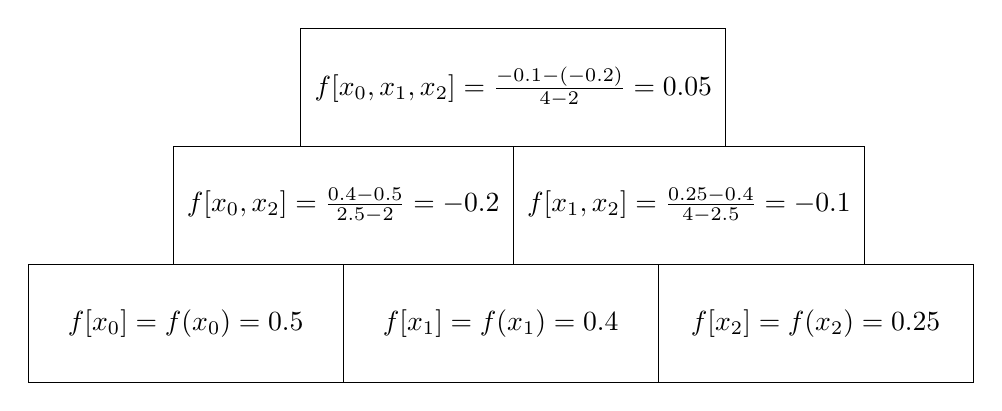
\begin{tikzpicture}[
        node distance = 0pt,
        every node/.style = {draw, minimum size=15mm, minimum width=40mm, inner sep=5pt, outer sep=0pt, anchor=center}
    ]
        \node (n1)  {$f[x_0, x_1, x_2] = \frac{-0.1-(-0.2)}{4-2}=0.05$};
%
        \node (n11) [below left=of n1.south]    {$f[x_0, x_2] = \frac{0.4-0.5}{2.5-2}=-0.2$};
        \node (n12) [right=of n11]              {$f[x_1, x_2] = \frac{0.25-0.4}{4-2.5}=-0.1$};
%
        \node (n21) [below left=of n11.south]   {$f[x_0]=f(x_0) = 0.5$};
        \node (n22) [right=of n21]              {$f[x_1]= f(x_1) = 0.4$};
        \node (n23) [right=of n22]              {$f[x_2] = f(x_2) = 0.25$};
    \end{tikzpicture}
\end{center}
\begin{equation*}
    P(x)= 0.5-0.2(x-2)+0.05(x-2)(x-2.5)
\end{equation*}

\section{Error of polynomial interpolation}\label{sec:error-of-polynomial-interpolation}

\begin{theorem}
    Let $f:[a,b] \to \mathbb{R}$ be at least $(n+1)$ times continuously differentiable and $P(x)$ be the interpolating polynomial of f in the nodes
    $x_0, \ldots, x_n \in [a,b]$ of degree $\leq n$.
    Then for every $x \in [a,b]$ there is a $\xi = \xi(x) \in [a,b]$ such that
    \begin{equation*}
        f(x)-P(x) = \underbrace{(x-x_0)(x-x_1)\ldots(x-x_n)}_{\coloneqq W_{n+1}(x)}\frac{f^{n+1}(\xi)}{(n+1)!}
    \end{equation*}
\end{theorem}
\begin{proof}
    Let $F(x) \coloneqq f(x)-p(x)-k*W_{n+1}(x)$ and select some $\hat{x}\in [a,b], \hat{x} \neq x_i$.
    We choose K such that $F(\hat{x})=0$.
    This is always possible since $W_{n+1}(x) \neq 0$. $F(x)$ has therefore $n+2$ roots.
    This means that $F'(x)$ has $n+1$ roots, $F''(x)$ has n roots etc., until $F^{n+1}(x)= f^{n+1}(x)-k(n+1)!$ has one root,
    which we call $\xi = \xi(\hat{x})$
    \begin{align*}
        0 &= f^{n+1}(\xi)-k*(n+1)! \\
        k &= \frac{f^{n+1}(\xi)}{(n+1)!}
    \end{align*}
\end{proof}
\begin{remark}
    In order to estimate the error, one needs to know the boundaries of the $(n+1)$th derivative on $[a,b]$
\end{remark}


\section{Chebyshev/Tschebyscheff-polynomials}\label{sec:chebyshev/tschebyscheff-polynomials}
If we have the freedom to choose the nodes $x_i$, then this can be used to minimize $\lvert W_{n+1}(x) \rvert$ and thus
the error of the interpolating polynomial.
We constrict ourselves to $[a,b] = [-1,1]$.
If  $[a,b] \neq [-1,1]$ then the transformation
\begin{align*}
[-1,1]
    &\to [a,b]\\
    x &\to \frac{a+b}{2}+x \frac{b-a}{2}=y
\end{align*}
with the inverse transformation
\begin{align*}
[a,b]
    &\to [-1,1]\\
    y &\to \frac{2y}{b-a}- \frac{a+b}{b-a}=x
\end{align*}
does not change the properties of the interpolation and approximation.
The Chebyshev polynomials are recursively defined by
\begin{align*}
    T_0(x) &= 1\\
    T_1(x) &= x\\
    T_{n+1} &= 2x*T_n(x)-T_{n-1}(x)
\end{align*}
This implies $T_n (x)= \cos(n*\arccos(x))$
\begin{proof}
    \begin{align*}
        T_{n+1} &= 2x*\cos(n*\arccos(x))-\cos((n-1) \arccos(x))\\
        &= 2\cos (\arccos(x))*\cos(n*\arccos(x))-\cos((n-1))\underbrace{\arccos((x)}_\varphi)\\
        &= \cos((n+1) \varphi)+\cos((n-1)\varphi)-\cos((n-1)\varphi) = \cos((n+1) \varphi)
    \end{align*}
\end{proof}

Properties of $T_n$:
\begin{itemize}
    \item the roots of $T_n$ are $\cos(\frac{2k+1}{2k}*\pi)$ $(k=0,\ldots, n-1)$
    \item $T_n\left(\cos(\frac{k*\pi}{n})\right)= (-1)^k$
    \item $\lvert T_n(x) \rvert \leq 1$ for $x \in [-1,1]$
\end{itemize}
\begin{align*}
    T_0(x) &= 1\\
    T_1(x) &= x\\
    T_2(x) &= 2x^2-1\\
    T_3(x) &= 4x^{3}-3x\\
    T_4(x) &= 8x^4-8x^2+1
\end{align*}
\begin{theorem}
    From all possible $(x_0, \ldots, x_n)^T \in [-1,1]^n \subset \mathbb{R}^n$ the value $\max_{x \in [-1,1]} \lvert w_{n+1}(x) \rvert$ becomes minimal if the nodes $x_i$ are
    the roots of the $(n+1)$st Chebyshev polynomial $T_{n+1}$
    \begin{align*}
        x_i &= \cos\left(\frac{2i+1}{2n+2} \pi\right), i=0,\ldots,n\\
        \text{Then } w_{n+1}(x) &= \frac{1}{2^n}* T_{n+1}(x) \\
        \text{and } \max_{x \in [-1,1]} \lvert w_{n+1}(x) \rvert &= \frac{1}{2^n}
    \end{align*}
\end{theorem}

\begin{proof}
    \begin{lemma}
        Let $q(x)=2^{n-1}x^n+\ldots$  be a polynomial unequal to the nth Chebyshev polynomial $T_n$.
        Then:
        \begin{equation*}
            \max_{x \in [-1,1]} \lvert q(x) \rvert > 1= \max_{x \in [-1,1]} \lvert T_n(x) \rvert
        \end{equation*}
        We assume $\lvert q(x) \rvert \leq 1$ for all $x \in [-1,1]$, $T_n(1) = 1$, $T_n\left( \cos \frac{\pi}{n} \right) = -1$.
        We consider $T_n(x)-q_n(x)$ at $[\cos \frac{\pi}{n}, 1]$.
        $q(x)$ and $T_n(x)$ have the same highest order coefficient $(2^{n-1})$.
        Therefore $T_n(x)-q(x)$ is of degree $n-1$
        \begin{align*}
            &\lvert q(x) \rvert \leq 1\\
            &\to T_n(1)-q(1) \geq 0\\
            &\to T_n\left(\cos \left( \frac{\pi}{n} \right) \right) - q\left(\cos \left( \frac{\pi}{n} \right) \right) \leq 0
        \end{align*}
        $T_n(x)-q_(x)$ has at least one root on $[\cos\frac{\pi}{n}, 1]$.
        In the same way, we can show that $T_n(x)-q(x)$ has at least one root on $[\cos\frac{2\pi}{n},\cos\frac{\pi}{n}]$
        and on $[\cos\frac{3\pi}{n},\cos\frac{2\pi}{n}]$ and on \ldots{} and on $[-1, \cos \left( \frac{(n-1)  \pi}{n} \right)]$.
        Therefore $T_n(x)-q(x)$ has n roots in $[-1,1]$.
        If the root is situated on the boundary of two sub intervals, then it's a double root, since $T_n(x)$ and $q(x)$ extremal.
        However $T_n(x) - q(x)$ is only of degree $\leq n-1$
        \begin{align*}
            T_n(x)-q(x) = 0 \text{ (!) contradicition to assumption } T_n(x) \neq q(x) \\
            \to \max_{x \in [-1,1]} \lvert w_{n+1}(x) \rvert = \frac{1}{2^n}
            \underbrace{\max_{x \in [-1,1]} \lvert \underbrace{2^n w_{n+1}(x)}_{T_{n+1}(x)} \rvert}_{ \geq 1 \text{ with Lemma}}\\
            \max_{x \in [-1,1]} \lvert w_{n+1}  \rvert \geq \frac{1}{2^n} \text{ with equality if } w_{n+1}(x) = \frac{1}{2^n}*T_{n+1}(x)
        \end{align*}
    \end{lemma}
\end{proof}


\section{hermite interpolation}\label{sec:hermite-interpolation}
If in addition to the values of $f$ also the values of the derivative $f'$ are known, we can construct the hermite interpolating polynomial.
Every node $x_i \in \{ x_0, \ldots, x_n \}$ corresponds to $2$ conditions which implies that the interpolating polynom is of degree $2n+1$

\begin{theorem}
    Let $f \in C^1([a,b])$ and $x_0, \ldots, x_n \in [a,b]$ pairwise distinct.
    Then the only polynomial of degree $2n+1$ that equals $f$ and $f'$ in $x_0, \dlots, x_n$ is given by
    \begin{align*}
        \HO_{2n+1}(x) &= \sum_{j=0}^{n} f(x_j) * \HO_{n,j}(x) + \sum_{j=0}^{n} f'(x_j) * \widehat{\HO}_{n,j}(x)\\
        \text{where } \HO_{n,j}(x) &= [1-2(x-x_j) * L'_{n,j}(x_j)]*L_{n,j}(x)^2\\
        \text{and } \widehat{\HO}_{n,j}(x) &= (x-x_j)*L_{n,j}(x)^2
    \end{align*}
    Here $L_{n,j}(x)$ are the Lagrange polynomials.
    It's easy to see that $\HO_{n,j}(x_i) = \delta_{ij}$ ($L_{n,j}(x_i) = \delta_{ij}$)
    and $\widehat{\HO}_{n,j}(x_i) = 0$ $\forall x_i$

    \begin{align*}
        \HO_{n,j}'(x) &= -2 L'_{n,j}(x_j)*L_{n,j}(x)^2 + 2[1-2(x-x_j)L_{n,j}'(x_j)]*L_{n,j}'(x)*L_{n,j}(x)\\
        \HO_{n,j}'(x_j) &= -2L_{n,j}'(x_j)+2L_{n,j}'(x_j) = 0\\
        H_{n,j}(x_i) |_{i \neq j} &= 0\\
        \\
        \widehat{\HO}_{n,j}'(x)&=L_{n,j}(x)^2+2(x-x_j)L_{n,j}'(x)L_{n,j}(x)\\
        \widehat{\HO}_{n,j}'(x_j)&= 1\\
        \widehat{\HO}_{n,j}'(x_i) |_{i \neq j} &= 0
    \end{align*}
\end{theorem}


    In summary we obtain
\begin{align*}
    \HO_{2n+1}(x) = \sum_{j=0}^{n} f(x_j)*\HO_{n,j}(x)+ \sum_{j=0}^{n} f'(x_j) \widehat{\HO}_{n,j}(x)
\end{align*}
\begin{center}
    \begin{tabular}{c c}
        \[ \HO_{n,j}(x_i) = \delta_{ij}\] & \[\HO_{n,j}'(x_i) = 0\]                      \\
        \[ \widehat{\HO}_{n,j}(x_i) = 0\] & \[ \widehat{\HO}_{n,j}'(x_i) = \delta_{ij}\]
    \end{tabular}
\end{center}
However, the construction by means of Lagrange polynomials is computationally expensive.
Again, divided differences are useful.
From the remainder of polynomial interpolation it follows:
\begin{lemma}
    Let $f \in C^n([a,b])$ and $X_0, \ldots, x_n$ be pairwise distinct in $[a,b]$.
    Then there is a $\xi \in [a,b]$ such that
    \begin{equation*}
        f[x_0,\ldots, x_n] = \frac{f^{(n)}(x)}{n!} \text{ (\textasteriskcentered)}
    \end{equation*}
\end{lemma}
\begin{proof}
    If $n+1$ nodes $x_0, \ldots, x_n$ and the values $f(x_i), f'(x_i)$ $(i=0, \ldots, n)$ are given, we define a sequence
    \begin{equation*}
        \hat{x}_{2i} = \hat{x}_{2i+1} = x_i
    \end{equation*}
    We generate divided differences with sequence.
    Obviously
    \begin{equation*}
        f[\hat{x_}{2i}, \hat{x}_{2i+1}]
        = \frac{f[\hat{x}_{2i+1}]-f[\hat{x}_{2i}]}{\hat{x}_{2i+1}-\hat{x}_{2i}}
    \end{equation*}
    can not be used.
    But considering $(\textasteriskcentered)$ and
    \begin{equation*}
        \lim_{x_A \to x_0} f[x_0, x_A] = f'(x_0)
    \end{equation*}
    it is justified to use the substitution
    \begin{equation*}
        f[\hat{x}_{2i}, \hat{x}_{2i+1}] = f'(x_i)
    \end{equation*}
    and use $f'(x_0), f'(x_1), f'(x_2), \ldots, f'(x_n)$ for
    $f[\widehat{x_0}, \widehat{x_1}], f[\widehat{x_2}, \widehat{x_3}] f[\widehat{x_4}, \widehat{x_5}],
    \ldots, f[\widehat{2n}, \widehat{x_{2n+1}}]$
    The remaining divided differences are generated as before.
\end{proof}

\section{Spline interpolation}\label{sec:spline-interpolation}
Although an interpolating polynomial can always be found, this is often not a very good approximation, especially in the case of large n.
Fluctuation in a small region can lead to great changes throughout the entire interval.
Piecewise interpolation can be preferable.

The simplest version of piecewise interpolation would employ polynomials of degree 1.
This has the big disadvantage that the resulting curve is not smooth/differentiable.
Better choice: Piecewise hermite interpolation with polynomials of degree 3.
A cubic spline interpolating function is a function $s$ with the properties
\begin{itemize}
    \item $s$ is a cubic polynomial labeled $s_j$ on the subinterval $[x_j, x_{j+1}]$
    \item $s_j(x_j) = f(x_j)$ for $j = 0, \ldots, n$
    \item $s_{j+1}(x_{j+1}) =s_j(x_{j+1})$
    \item $s_{j+1}'(x_{j+1}) =s_j'(x_{j+1})$
    \item $s_{j+1}''(x_{j+1}) =s_j''(x_{j+1})$
    \item one of the following boundary conditions
    \begin{itemize}
        \item $s''(x_0)=s''(x_n) = 0$ (free boundary)
        \item $s'(x_0) = f'(x_0)$ and $s'(x_n) = f'(x_n)$ (hermite boundary)
    \end{itemize}
\end{itemize}


\chapter{Trigonometric interpolation}\label{ch:trigonometric-interpolation}
We consider the n-dimensional space $T_c^{n-1}$ of complex trigonometric polynomials
\begin{align*}
    \Phi_n(x) = \sum_{k=0}^{N-1} c_k * e^{ikx} \text{ with } c_k \in \mathbb{C}
\end{align*}
of degree $N-1$.
These polynomials are periodic: $\Phi_n(x)=\Phi_n(2 \pi + x)$.
The linear independence of the basis functions $e^{ikx}$ guarantees that for $N$ data-points $(x_j, f_j)$ with $j= 0, \ldots, N-1$ there is exactly
one interpolating polynomial $\Phi_n$ with $\Phi_n(x_j)=f_j$.
If we constrain ourselves to equidistant nodes $x_j = \frac{2  \pi j}{N}$ then we obtain the Vandermond-System.
\begin{equation*}
    \begin{pmatrix}
        1      & w_0     & w_0^2     & \dots  & w_0^n         \\
        \vdots & \vdots  & \vdots    & \ddots & \vdots        \\
        1      & w_{n-1} & w_{n-1}^2 & \dots  & w_{n-1}^{n-1}
    \end{pmatrix}
    *
    \begin{pmatrix*}
        c_0\\
        \vdots \\
        c_{n-1}
    \end{pmatrix*}
    =
    \begin{pmatrix*}
        f_0\\
        \vdots\\
        f_{n-1}
    \end{pmatrix*}
\end{equation*}
where $w_k$ are the roots of unity of degree $N$.
\begin{align*}
    w_k \coloneq e^{ikx} &= e^{i*2 \pi k / N}\\
    (w_k)^N &= 1
\end{align*}
\begin{lemma}
    The basis functions $e^{ikx}$ are orthogonal with respect to the inner product
    \begin{equation*}
        \langle f, g \rangle \coloneq \frac{1}{n} * \sum_{j=0}^{N-1} f(x_j) * \overline{g(x_j)}
    \end{equation*}
    with the nodes $x_j = {2\pi j}/{N}$
\end{lemma}
\begin{proof}
    \begin{align*}
    (w_k)
        ^l &= (w_l)^k = w_1^{k*l}\\
        \left( e^{i*2 \pi k / N} \right)^l &= \left( e^{i*2 \pi l / N} \right)^k = e^{i*2 \pi kl / N}\\
        \\
        \langle e^{ikx}, e^{ilx} \rangle &= \frac{1}{N} * \sum_{j=0}^{N-1} e^{i*2 \pi k j / N} * e^{-i*2 \pi l j / N}\\
        &= \frac{1}{n} \sum_{j=0}^{N-1} \underbrace{w_j^m w_j^{-l}}_{w_j^{k-l}} = N * d_{kl} \text{ is equivalent to}\\
        \sum_{j=0}^{N-1}w_j^k &= \sum_{j=0}^{N-1} w_k^{j} = N * \delta_{k0}
    \end{align*}
    Roots of unity $w_k$ are solutions of $0 = w^n-1 = (w-1)(w^{n-1}+w^{n-2}+\ldots+1) = (w-1) \sum_{j=0}^{N-1} w_k^j$
    If $k \neq 0$ then $w_k \neq 1$ and therefore $\sum_{j=0}^{N-1} w_k^j = 0$.
    If $k=0$ then $\sum_{j=0}^{N-1} w_k^j = N$.
    The coefficients $c_n$ of the trigonometric interpolation of the $N$ data points $(x_l, f_l)$ with equidistant nodes $x_l = \frac{2 \pi l}{N}$ are given by
    \begin{align*}
        c_k &= \sum_{l=0}^{N-1} f_l * w_l^{-k} \text{ for } k = 0, \ldots, N-1\\
        &= \langle f, e^{ikx} \rangle
    \end{align*}

    Proof by insertion:
    \begin{align*}
        \Phi(x_m)=\sum_{k=0}^{N-1} c_k *w_m^k &= \sum_{k=0}^{N-1} \frac{1}{N} \sum_{l=0}^{N-1} f_l * w_l^{-k} w_m^k\\
        &= \frac{1}{N} \sum_{l=0}^{N-1} f_l \sum_{k=0}^{N-1} \underbrace{w_l^{-k}*w_m^k}_{w_k^{m-l}}\\
        &= \frac{1}{N} \sum_{l=0}^{N-1} f_l * N * \delta_{ml} = f_m
    \end{align*}
\end{proof}
\begin{remark}
    If the polynomial is real
    \begin{equation*}
        \phi_N(x) = \sum_{k=0}^{N-1}c_{k}*e^{ikx} \in \mathbb{R} \text{ for all } x \in \mathbb{R}
    \end{equation*}
    one can use the representation
    \begin{align*}
        \text{for odd N: }\Phi_{2n+1}(x) &= \frac{a_0}{2}+\sum_{k=1}^{n} a_k * \cos(kx) + b_k * \sin(kx) \text{ with } n = \frac{N-1}{2}\\
        \text{for even N: } \Phi_{2n}(x) &= \frac{a_0}{2}+\sum_{k=1}^{n-1} a_k * \cos(kx) + b_k * \sin(kx) + \frac{a_n}{2} * \cos(nx) \text{ with } n = \frac{N}{2}
    \end{align*}
    with $a_k, b_k \in \mathbb{R}$.
    It is $a_k = c_k + c_{N-k}$ and $b_k = i *(c_k-c_{N-k})$
\end{remark}
\begin{remark}
    With $c_{-j} = c_{N-j}$ we can write for odd N
    \begin{align*}
        \Phi_n(x_l) = \sum_{k=0}^{N-1} c_k e^{ikx_l} = \sum_{k = -n}^{n} c_k *e^{ikx_l}  
        \text{ with } n = \frac{N-1}{2}\\
        e^{-ikx_l} = e^{-ik \frac{2 \pi l}{n}} = e^{-i k \frac{2 \pi l}{N}} * \underbrace{e^{i 2 \pi l}}_{=1^l}
        = e^{i (N-k) \frac{2 \pi l}{N}}
    \end{align*}
    Strong similarity to truncated Fourier series:
    \begin{equation*}
        f_n(x) = \sum_{k = -n}^{n} \widehat{f_k} * e^{ikx}
    \end{equation*}
    with coefficients
    \begin{equation*}
        \widehat{f_k} = \frac{1}{2 \pi } \integral{0}{2 \pi}{f(x) * e^{-ikx}}
    \end{equation*}
    If the integral is approximated as a sum of the x values $x_l = \frac{2 \pi l}{N}$ one
    obtains an approximation of $\widehat{f_k}$
    \begin{align*}
        \integral{0}{2 \pi}{g(x)} \approx \frac{2 \pi }{N} \sum_{k = 0}^{N-1}g(x_k)\\
        \widehat{f_k} \approx \frac{1}{N} \sum_{l = 0}^{N-1} f_l e^{-ikx_l} = \frac{1}{N}
        \sum_{l=0}^{N-1} e^{-ikl \frac{2 \pi}{N}} f_l = c_l
    \end{align*}
    Therefore the isomorphism
    \begin{equation*}
        \widetilde{f_n}: \mathbb{C} \to \mathbb{C}: (f_j) \to (\c_j)
    \end{equation*}
    is also called discrete Fourier-Transformation.
    \begin{align*}
        c_k = \frac{1}{N} \sum_{l=0}^{N-1} f_l e^{-i 2 \pi k l / N}\\
        f_k = \sum_{l=0}^{N-1} c_l e^{i 2 \pi k l / N}
    \end{align*}
\end{remark}


    \section{Fast Fourier Transformation}\label{sec:fast-fourier-transformation}
The calculation of the coefficients $c_k$ from the function values
$f_k$ (or inverse operation) is a matrix-vector iultiplication, and therefore,
they require $ \propto N^2$ operations.
There is an algorithm that only needs $\propto N \log N$ operations.
If $N$ is even $M = N/2$ and $w = \exp\left(\frac{-i 2 \pi }{N}\right)$ then the trigonometric
sums
\begin{align*}
    \alpha_k = \sum_{l=0}^{N-1} f_l w^{kl} \text{for } k = 0, \ldots, N-1
\end{align*}
can be written as
\begin{align*}
    \xi&: w^2, m = 0, \ldots, M-1\\
    \alpha_{2m} &= \sum_{l=0}^{M-1} g_l * \xi ^{ml} \text{with } g_l = f_l + f_{l+m}\\
    \alpha_{2m+1} &= \sum_{l=0}^{M-1} h_l * \xi^{ml} \text{with } h_l = (f_l - f_{l+m}) * w^l
\end{align*}
\begin{proof}
    \begin{align*}
        \alpha_{2m} &= \sum_{l=0}^{N-1} f_l w^{2ml}\\
        &= \sum_{l=0}^{N/2-1}f_l * w^{2ml} + f_{l + N/2} w^{2(l+N/2)m}\\
        &= \sum_{l=0}^{N/2-1}(f_l + f_{l+N/2}) * (w^2)^{lm}\\
        \alpha_{2m+1} &= \sum_{l=0}^{N-1} f_l w^l/(2m+1)\\
        &= \sum_{l=0}^{N/2-1} f_{l} * w^{l/(2m+1)}+ f_{l + N/2} * w^{l + N/2}\\
        &= \sum_{l=0}^{M-1} (f_l- f_{l+M}) w^l * (w^2)^{lm}
    \end{align*}
\end{proof}
If the initial number of points/terms of the sums $N$ is a power of two, the process can be repeated,
until there is only one term left.

This can be done on a single vector by overwriting the old values because the number of terms
stays constant $\{ f_0, f_1, \ldots, f_{n-1} \} \to \{ g_0, \ldots, g_{N/2-1}, h_0, \ldots, h_{N/2}-1$
and two f-values always form one g and one h value.
TODO[Scheme]
For every reduction $\propto $ N Operations are needed and there are $ N \log_{2} N$ \textrightarrow
$N * \log_2 N$ total operations.

\chapter{least-square approximation}\label{ch:least-square-approximation}
We have seen that any set of points $(x_i, y_i)$ $i = 1, \ldots, n$ with pairwise distinct $x_i$ can be interpolated by polynomial of degree $\leq n-1$.
However, in most cases, the underlying mathematical or physical relationship does not justify the use of a high-order polynomial.
It is also not imperative to match each point exactly since the data usually carry errors.
Instead, it is desirable to find a simple function(e.g.\ a polynomial) of low order and allow for small discrepancy with the data.

Different definitions of ``discrepancy'' are conceivable.
\begin{equation*}
    E_{\infty} = \max_{i=1,\ldots,n} \{ |f(x_i) - y_i| \}
\end{equation*}
Determining f such that $E_\infty$ is minimal will provide a function f which has the smallest possible maximal deviation from the data.
\begin{equation*}
    E_1 = \sum_{i=1}^n |f(x_i) - y_i|
\end{equation*}
Minimalizing $E_i$ leads to an $f$ where the sum of all absolute deviations from the data is minimal.
\begin{equation*}
    E_2 = \sqrt{\sum_{i=1}^n |f(x_i) - y_i|^2}
\end{equation*}
Minimizing $E_2$ (i.e.\ minimizing $E_2^2$) will produce a function $f$ with the least squared deviation from the data.
\begin{equation*}
    E_p = \left( \sum_{i=1}^n |f(x_i) - y_i|^p \right)^{\frac{1}{p}}
\end{equation*}
Each approach has its applications.
In most cases $E_2$ is used.
This is based on the assumption that measurements are distributed around the true value according to Gaussian distribution.
Assume that we have measured a data-vector $\{ y_i \}$ and try to find a model m represented by a function $f_m$ (e.g., a polynomial of degree 1).
We try to maximize $"W(m \vert \{ y\})$, i.e.\ the likelihood for for $m$ under the condition that $\{ y \}$ has been measured.
\begin{align*}
    \text{Bayes-theorem: } W(m \vert \{ y \}) &= \frac{W(\{ y \} \vert m) * W(m)}{W(\{ y \})} \\
\end{align*}
\begin{itemize}
    \item $W(\{ y\})$ is a constant (independent of m)
    \item $W(m)$ is the probability that we would choose a model $m$ if we had no data at all.
    Usually one does not discriminate different models a priory (beyond selecting a class of functions).
    $W(m)$ is therefore a constant.
    \item $W(\{y \} \vert m)$ is the probability that a given mode produces the data $\{ y \}$.
\end{itemize}
\begin{align*}
    W(\{ y \} \vert m) &= \prod_{i=1}^n \frac{1}{\sqrt{2 \pi \sigma^2}} \exp \left( - \frac{(y_i - f_m(x_i))^2}{2 \sigma^2} \right) \\
    &= \frac{1}{(2 \pi \sigma^2)^{\frac{n}{2}}} \exp \left( - \frac{1}{2 \sigma^2} \sum_{i=1}^n (y_i - f_m(x_i))^2 \right) \\
    &= \frac{1}{(2 \pi \sigma^2)^{\frac{n}{2}}} \exp \left( - \frac{1}{2 \sigma^2} E_2^2 \right) \\
\end{align*}
$ \to{} W(\{y\} | m)$ is maximal if $E_2$ is minimal.
If $W(\{y\} | m)$ is maximal usually $W(m | \{y\})$ is maximal as well.
$E_2^2 / \sigma^2$ is often denoted as $\chi^2$ ``chi-squared''.

\begin{remark}
    If $y_i$ carries a known error $\sigma_i$
    \begin{align*}
        W(\{y\} | m) &= \prod_{i=1}^n \frac{1}{\sqrt{2 \pi \sigma_i^2}} \exp \left( - \frac{(y_i - f_m(x_i))^2}{2 \sigma_i^2} \right)\\
        &= \prod_{i=1}^n \left( \frac{1}{\sqrt{2 \pi \sigma_i^2}} \right) \exp \left( - \underbrace{\sum_{i=1}^{n} \frac{(y_i - f_m(x_i))^2}{2 \sigma_i^2 \right)}}_{\chi^2 } \right) \\
    \end{align*}
\end{remark}
\begin{example}
    Simple case: $f(x) = ax + b$
    \begin{equation*}
        E_2^2 = \sum_{i=1}^{n}[y_1 - (ax_i + b)]^2
    \end{equation*}
    $E_2^2$ is minimal if
    \begin{align*}
        \frac{\partial E_2^2}{\partial a} &= \frac{\partial E_2^2}{\partial b} = 0\\
        0 = \frac{\partial }{\partial a} \sum_{i=1}^n [y_i - (ax_i + b)]^2 &= \sum_{i=1}^n -2x_i[y_i - (ax_i + b)] \\
        (i) \phantom{=} a \sum_{i=1}^n x_i y_i + b \sum_{i=1}^n x_i &= \sum_{i=1}^n x_i^2 y_i \\
        0 = \frac{\partial }{\partial b} \sum_{i=1}^{n} [y_i - (ax_i + b)]^2 &= \sum_{i=1}^n -2[y_i - (ax_i + b)] \\
        (ii) \phantom{=} a \sum_{i=1}^n x_i + b \sum_{i=1}^n 1 &= \sum_{i=1}^n y_i \\
    \end{align*}

    We can a define a Matrix to solve the problem:
    \begin{equation*}
        \begin{pmatrix}
            \sum_{i=1}^n x_i^2 & \sum_{i=1}^n x_i \\
            \sum_{i=1}^n x_i   & n                \\
        \end{pmatrix}
        *
        \begin{pmatrix}
            a \\
            b \\
        \end{pmatrix}
        =
        \begin{pmatrix}
            \sum_{i=1}^n x_i y_i \\
            \sum_{i=1}^n y_i     \\
        \end{pmatrix}
    \end{equation*}
\end{example}






\end{document}
